\chapter{Java静态安全扫描工具需求分析与设计}
\section{系统整体概述}

\section{系统需求分析}
\subsection{功能性需求}
\subsection{非功能性需求}
% 保密性、安全性、扩展性、健壮性、效率
\subsection{系统用例描述}
\section{系统总体设计}
本系统是一个结合污点分析,程序切片和LSTM的静态Java源代码扫描系统。系统总体架构如图~\ref{overview}所示,系统主要分为前端和后端两大部分,前端部分运行在用户端,包含用户界面模块、污点分析模块、程序切片模块、部分预测模块和预处理模块的泛化功能部分,而在扫描系统后端运行在服务器端,包含预处理模块的向量化功能部分,另一部分预测模块和数据库。


\begin{figure}[htb]
	\centering
	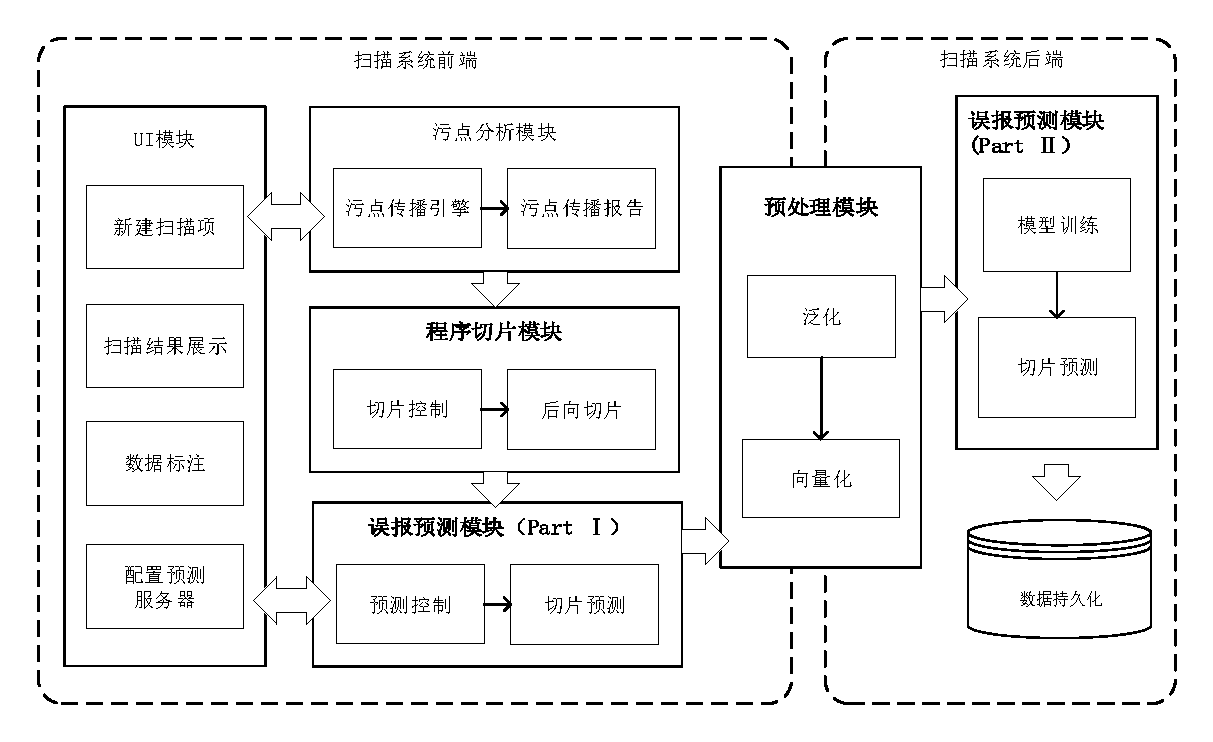
\includegraphics[width=5in]{FIGs/system-architecture.pdf}
	\caption{系统总体架构图}\label{overview}
\end{figure}

\section{污点分析模块设计}
\subsection{污点分析流程设计}

\section{程序切片模块设计}
\subsection{程序切片流程设计}

\section{数据预处理模块设计}
\subsection{数据预处理流程设计}

\section{误报预测模块设计}
\subsection{误报预测流程设计}

\section{UI模块设计}

\section{数据库设计}

\section{本章小结}